% fancytikzposter.tex, version 2.1
% Original template created by Elena Botoeva [botoeva@inf.unibz.it], June 2012
% 
% This file is distributed under the Creative Commons Attribution-NonCommercial 2.0
% Generic (CC BY-NC 2.0) license
% http://creativecommons.org/licenses/by-nc/2.0/ 
\documentclass{a0poster}
\usepackage[USenglish]{babel}% or british
\usepackage[T1]{fontenc}


\usepackage{wrapfig}
\usepackage{fancytikzposterM} 
\usepackage{multirow}
\usepackage{array}

% background picture
\usebackgroundtemplate{7}

\definecolor{myblue3}{HTML}{0C3E07}%main frames


\usepackage[margin=\margin cm, paperwidth=84.1cm, paperheight=118.9cm]{geometry}


\usepackage{cmbright}
%\usepackage[default]{cantarell}
%\usepackage{avant}
%\usepackage[math]{iwona}
\usepackage[math]{kurier}
\usepackage[T1]{fontenc}
\usepackage{tikz}

%%%%%%%%%%%%%%%%%%%%%%%%%%
%%% SET FONT SIZES %%%%%%%%%%%%%
%%%%%%%%%%%%%%%%%%%%%%%%%%
\renewcommand{\Huge}{\fontsize{64}{85}\selectfont} % Main title
\renewcommand{\huge}{\fontsize{44}{70}\selectfont} % Sub title
\renewcommand{\LARGE}{\fontsize{48}{48}\selectfont} % Box headers
\renewcommand{\Large}{\fontsize{42}{40}\selectfont} % Authors
\renewcommand{\normalsize}{\fontsize{40}{42}\selectfont} % Text in the boxes
\renewcommand{\footnotesize}{\fontsize{34}{42}\selectfont} % references
\newcommand{\footnotesizeminus}{\fontsize{31}{38}\selectfont} % references
\renewcommand{\small}{\fontsize{24}{22}\selectfont}
\newcommand{\smallest}{\fontsize{18}{16}\selectfont}
%% add your packages here


%% Set the folder that contains the images
\graphicspath{ {./Lowres/} }


\title{How much are wild vertebrate populations evolving right now?\vspace{-0.2em}}
\author{{\LARGE{Timoth\'{e}e Bonnet}, Michael Morrissey \& Loeske Kruuk}\\ \vspace{-20pt} \footnotesize Australian National University \& University of St Andrews
\\
}

\begin{document}

%%%%% ---------- the background picture ---------- %%%%%
%% to change it modify the macro \BackgroundPicture
%\ClearShipoutPicture
%\AddToShipoutPicture{\BackgroundPicture}

\noindent % to have the picture right in the center

\begin{tikzpicture}
  \initializesizeandshifts
  % \setxshift{15}
  \setyshift{2.5} % uncomment this line to condense the boxes

  \newcommand{\volesize}{0.8cm}

  %% the title block, #1 - shift, the default value is (0,0), #2 - width, #3 - scale
  %% the alias of the title block is `title', so we can refer to its boundaries later
  \ifthenelse{\equal{\template}{1}}{ 
    \titleblock[(-0.7,0)]{48}{1}
			}{
    \titleblock[(-10,0)]{87}{1.5}
			}
			
\addlogo[east]{(10,0)}{8cm}{loeske}
\addlogo[west]{(-10,0)}{8cm}{tim}

\coordinate (aaa) at (currenty);

	\blocknodew[($(currenty)+(19.6,0)$)]{77}{\textsc{The big problem:} We do not know how much wild organisms are currently evolving!}
		{Fisher's fundamental theorem of natural selection states that \textbf{additive genetic variation in fitness measures evolution across all traits and all the genome}. That is just what we need{\color{colorone}{\**}}!
		Yet, there are few estimates in free-ranging populations, and most may be unreliable. Indeed, it is difficult to measure fitness, difficult to estimate genetic variance, statistical models tend not to fit the data, and it is unclear how to interpret estimates from generalized linear models. We use a dozen long-term monitored populations with high quality fitness (measured as lifetime breeding success) and relatedness measurements to tackle these issues. How to make the most of these data? Are birds and mammals currently evolving? 
		}
	
%%%%%%%%%%%%%%%%%%%%%%%%%%%%%%%%%%%%%%%%%%%%%%%%%%%%%%%%%%%%%%%%%%%%%%%%%%%%%	
	\blocknodew[($(currenty)+(0,2)$)]{77}{\textsc{Theory:} How to estimate additive genetic variance in relative fitness ($V_A(\omega)$) ?}
	{	
	\hspace{-0.5cm}
		\begin{tabular}{p{0.30\textwidth} p{0.029\textwidth} p{0.30\textwidth} p{0.029\textwidth} p{0.30\textwidth}}
		
		\parbox{24cm}{\vspace{-0.3cm} \hspace{1cm} \textsc{Model distributions for fitness}\\
		
		 {\centering  \begin{tabular}{c}
		    \includegraphics[width=20cm]{Rgraph/figure/zidist-1.pdf}
		    \end{tabular}
		    
		    }
		     \footnotesize Zero-Inflated Over-Dispersed Poisson models tend to fit well lifetime fitness data. Quantitative genetic estimates may be more precise than with Gaussian or Poisson models.
		  }
		&

		&
		\parbox{24cm}{ \hspace{1cm} \textsc{Estimate latent genetic variation}\\
		
		   {\centering \begin{tabular}{c} 
		   \includegraphics[width=20cm]{Rgraph/figure/latentGmat-1.pdf}
		   \end{tabular}
		   
		   }
		   \footnotesize Quantitative genetic \textit{\textsc{animal models}} use relatedness matrix to estimate G-matrix for the zero-inflation and the over-dispersed Poisson processes on two latent scales (log and logit).
		  }
		&
		  
		&
		\parbox{24cm}{\textsc{Convert latent parameters to $V_A(\omega)$}\\
		
		{\centering \begin{tabular}{c}
		  \includegraphics[width=20cm]{Rgraph/figure/DlambdaZI-1.pdf}
		\end{tabular}
		
		}		
		\footnotesize Monte-Carlo integration of latent breeding values to the data scale. Back-transformation works for individual-based simulations: $V_A(\omega)$ equals the increase in population growth rate.
	      }
		\end{tabular}
		\vspace{-0cm}
	}%end block
%%%%%%%%%%%%%%%%%%%%%%%%%%%%%%%%%%%%%%%%%%%%%%%%%%%%%%%%%%%%%%%%%%%%%%%%%%%%%	
	\coordinate (tfirstcol) at (currenty);
	
 \coordinate (width) at ($(76.8,0) - (2.1,0)$);   
 %% the content of the block
          \draw let \p1=($(width)-(0,0)$) , \p2=($(0,\blocktitleheight cm)-(0,2.4cm)$)
          in node[draw, anchor=north, color=blocktitlefillcolor, text=blocktextcolor, 
          frame, rectanglesplittwo, rectangle split horizontal=false, 
          rectangle split part fill={blocktitlefillcolor, none}, %
          rectangle split empty part height= \y2 
          ]
          (box) at ($(currenty)+(0,2)$) {
            \nodepart{second}
            \begin{minipage}{\x1}
            \begin{center}
	      \vspace{34cm} % a very mesy trick to control box height...
            \end{center}
           \end{minipage}
          }; 

          %% the title of the block
          \node[frame, anchor=north west, text=blocktitletextcolor] at (box.north west)
          {\bf\LARGE \textsc{Emperical results:} Additive genetic variation in fitness detectable in most populations};
          
          \newcommand{\matpicw}{5.9cm}
          
          \node[anchor=north west] (map) at ($(box.north)+(0,-2.8)$) {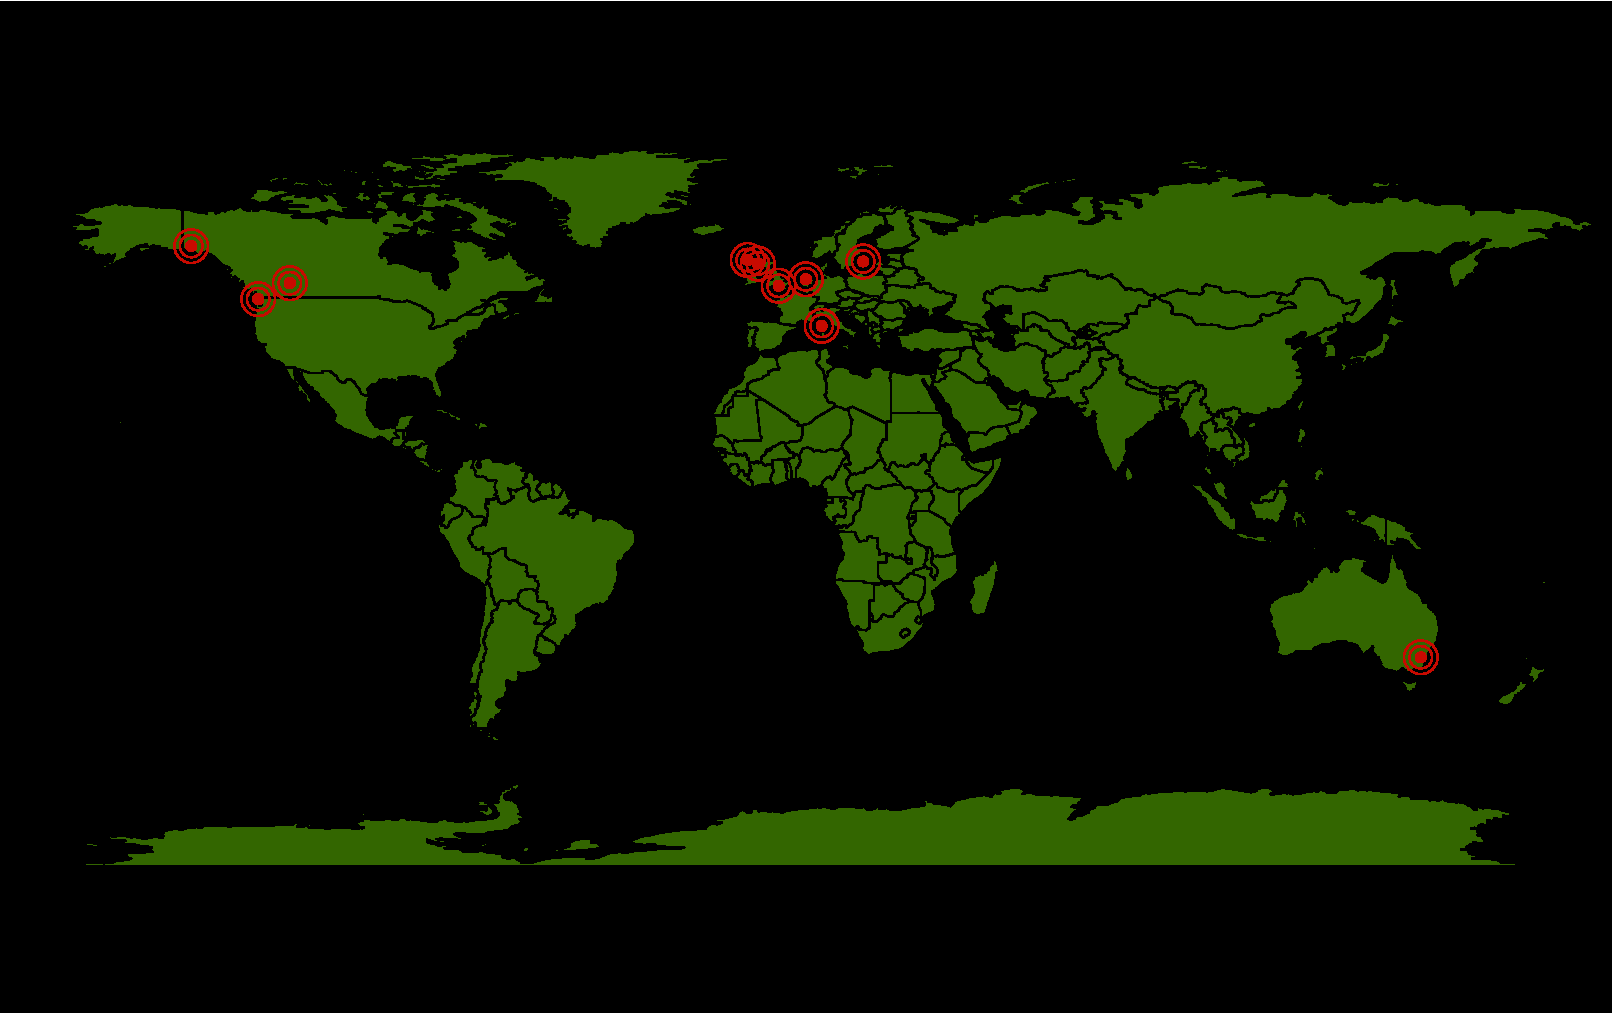
\includegraphics[height=13.2cm, trim=0cm 4.5cm 0cm 2.5cm, clip]{Rgraph/map.pdf}};
	  \node[anchor=north west] (pictab) at ($(box.north west)+(0,-3.3)$) {
	  \setlength{\tabcolsep}{12pt}

	  \begin{tabular}{c c c c c c c c c c c}
	    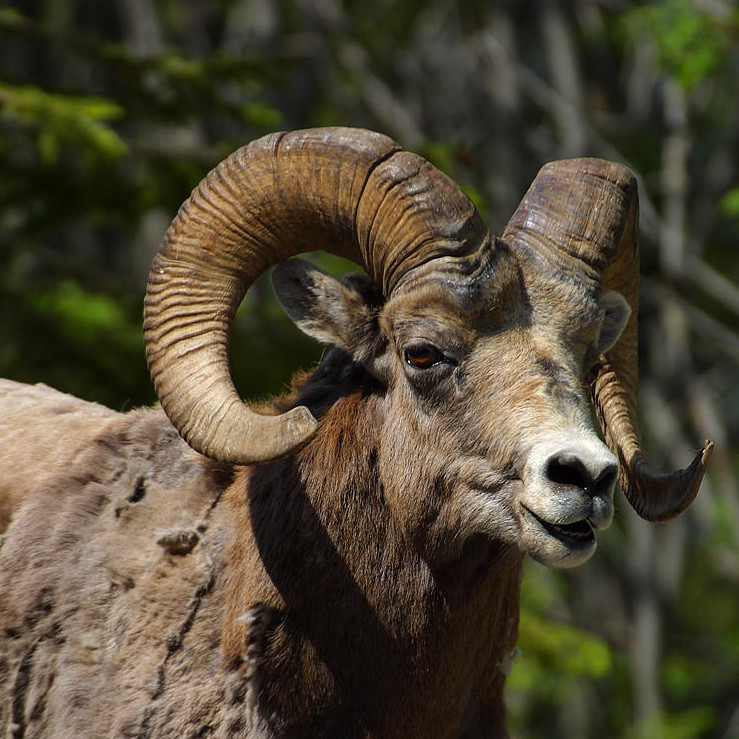
\includegraphics[width=\matpicw]{bhs} & 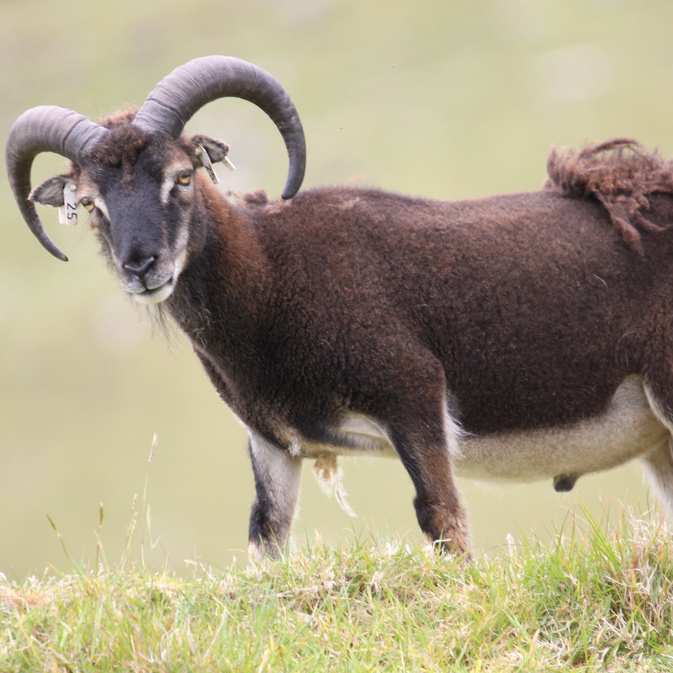
\includegraphics[width=\matpicw]{soay} &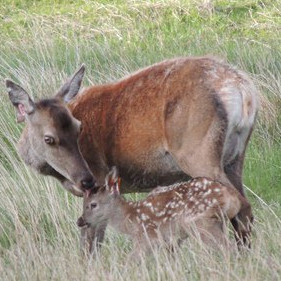
\includegraphics[width=\matpicw]{doe} & 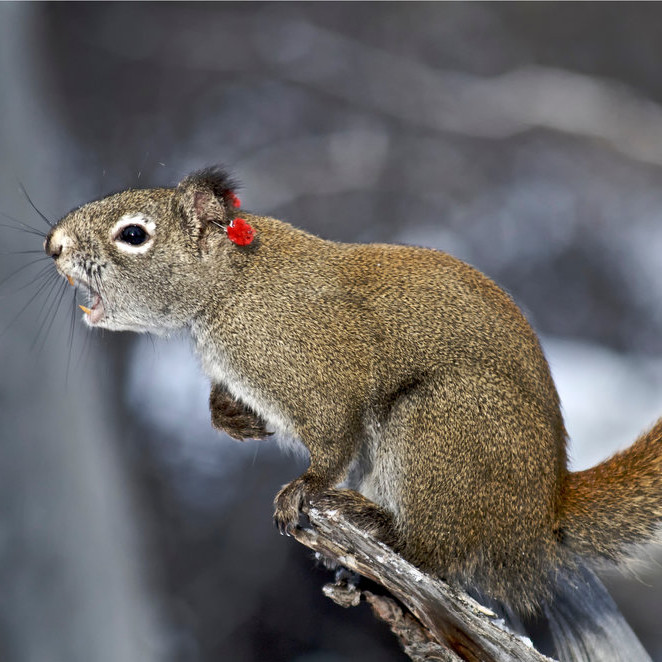
\includegraphics[width=\matpicw]{squirrel}&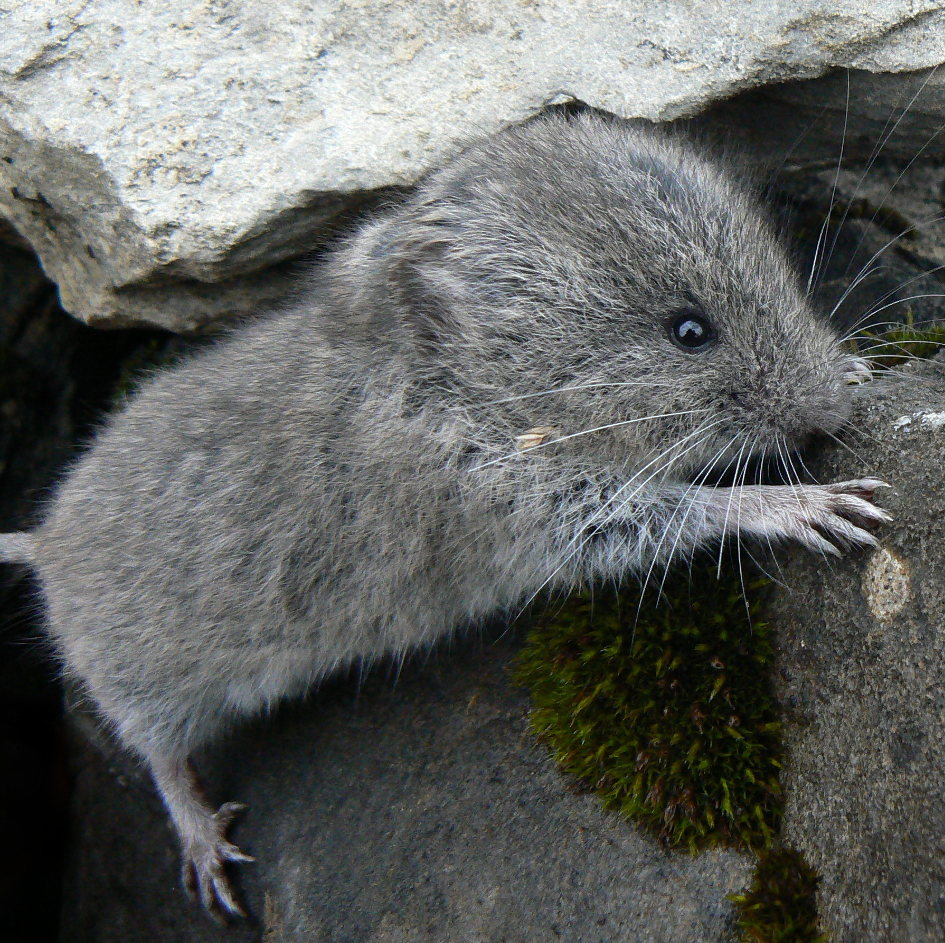
\includegraphics[width=\matpicw]{vole} \\ 
	   % 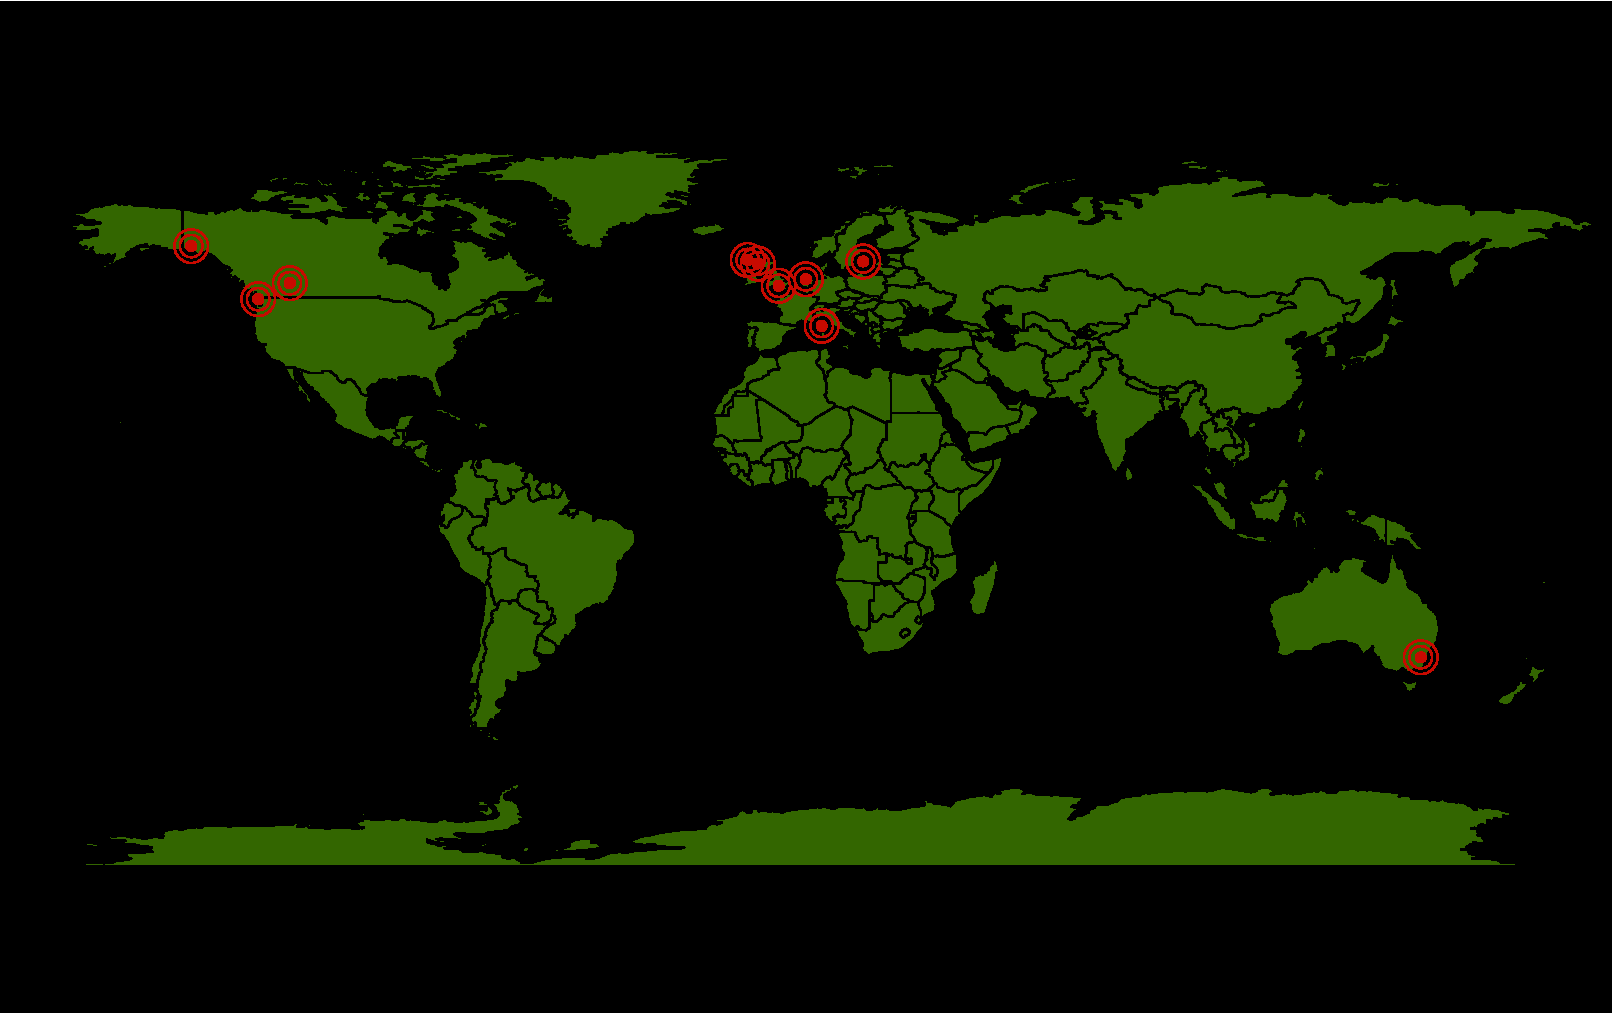
\includegraphics[height=\matpicw, trim=0.5cm 4.5cm 0.5cm 2.5cm, clip]{Rgraph/map.pdf} &
	    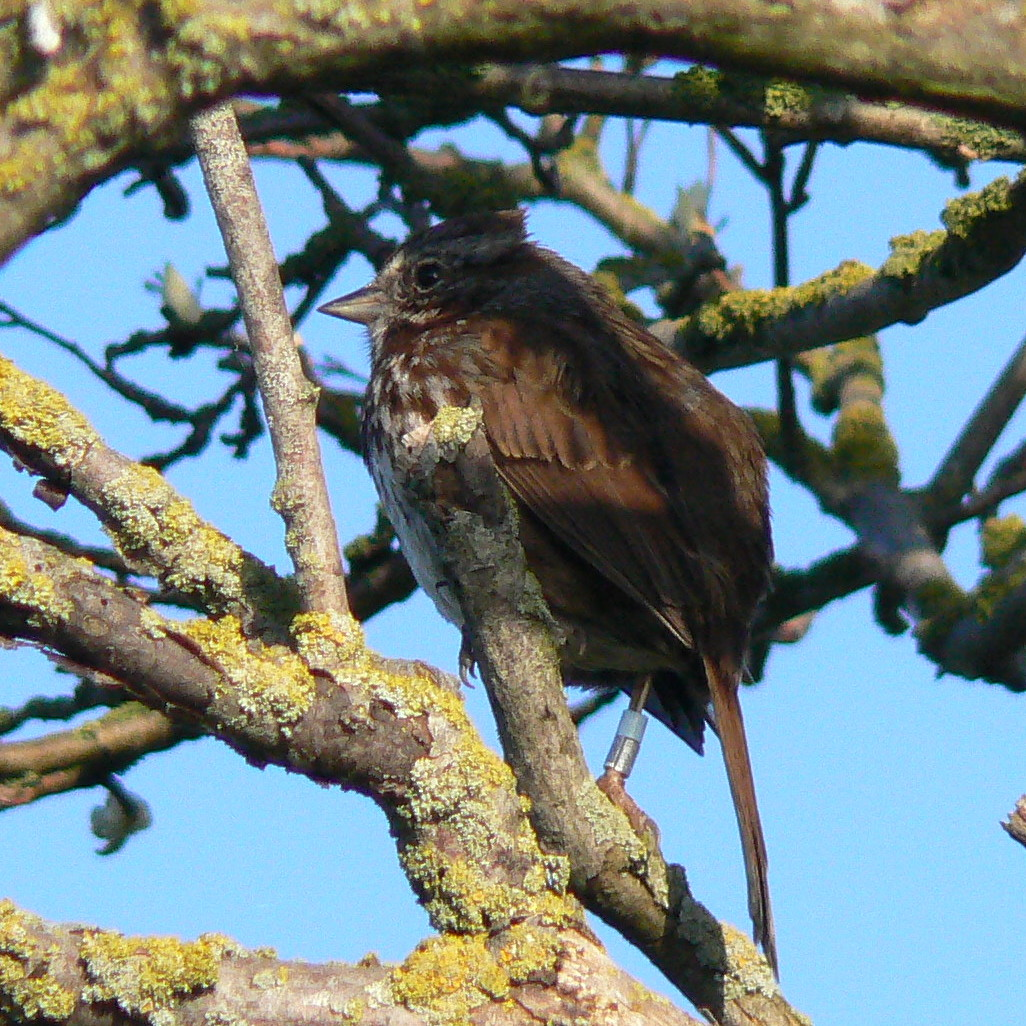
\includegraphics[width=\matpicw]{ssp} & 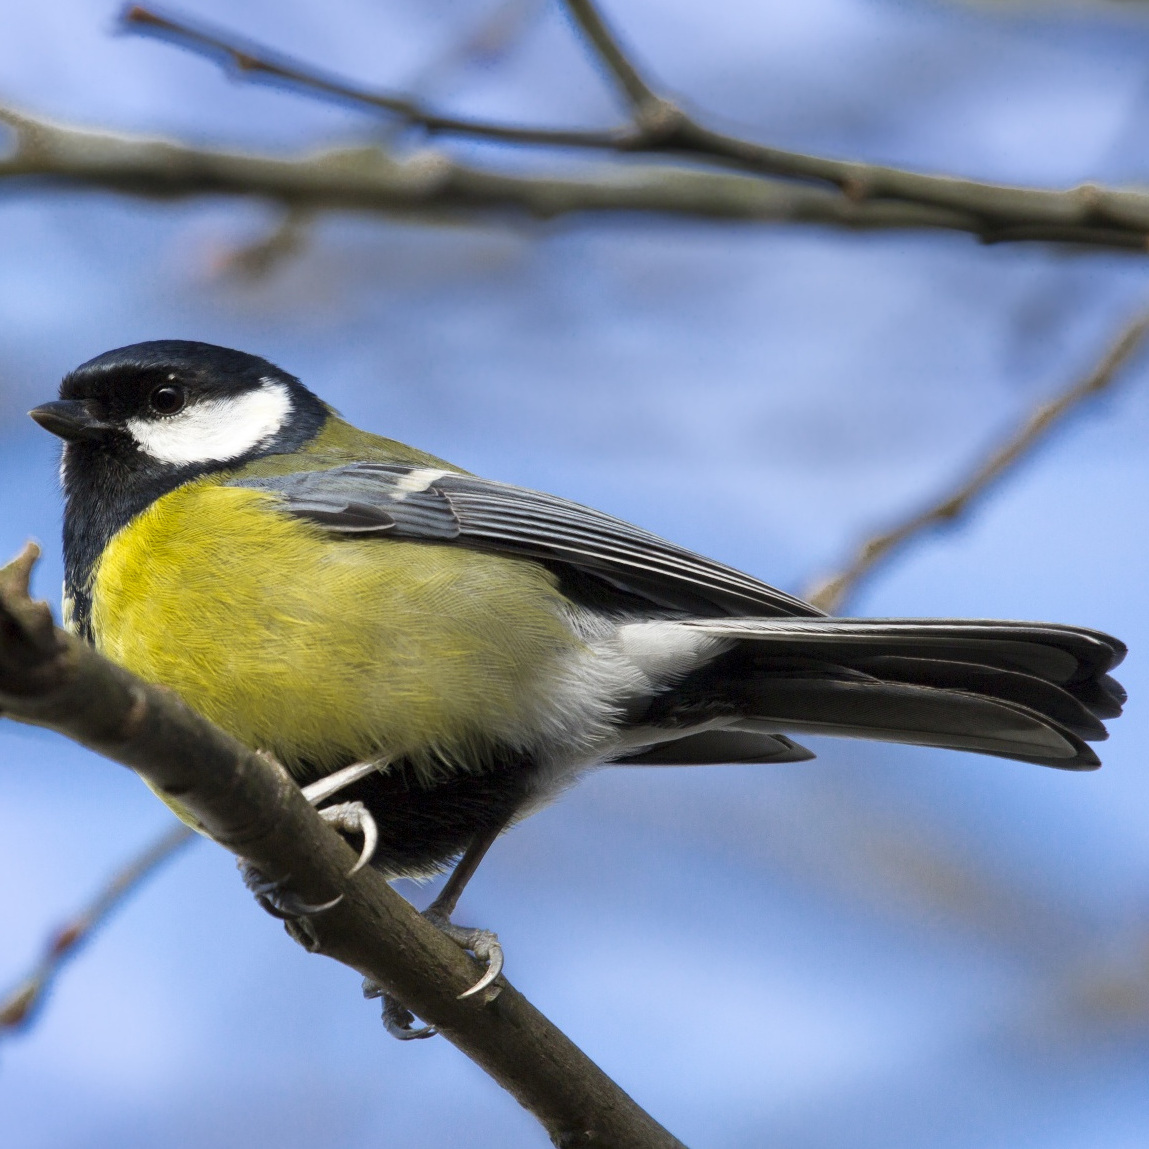
\includegraphics[width=\matpicw]{gt2} &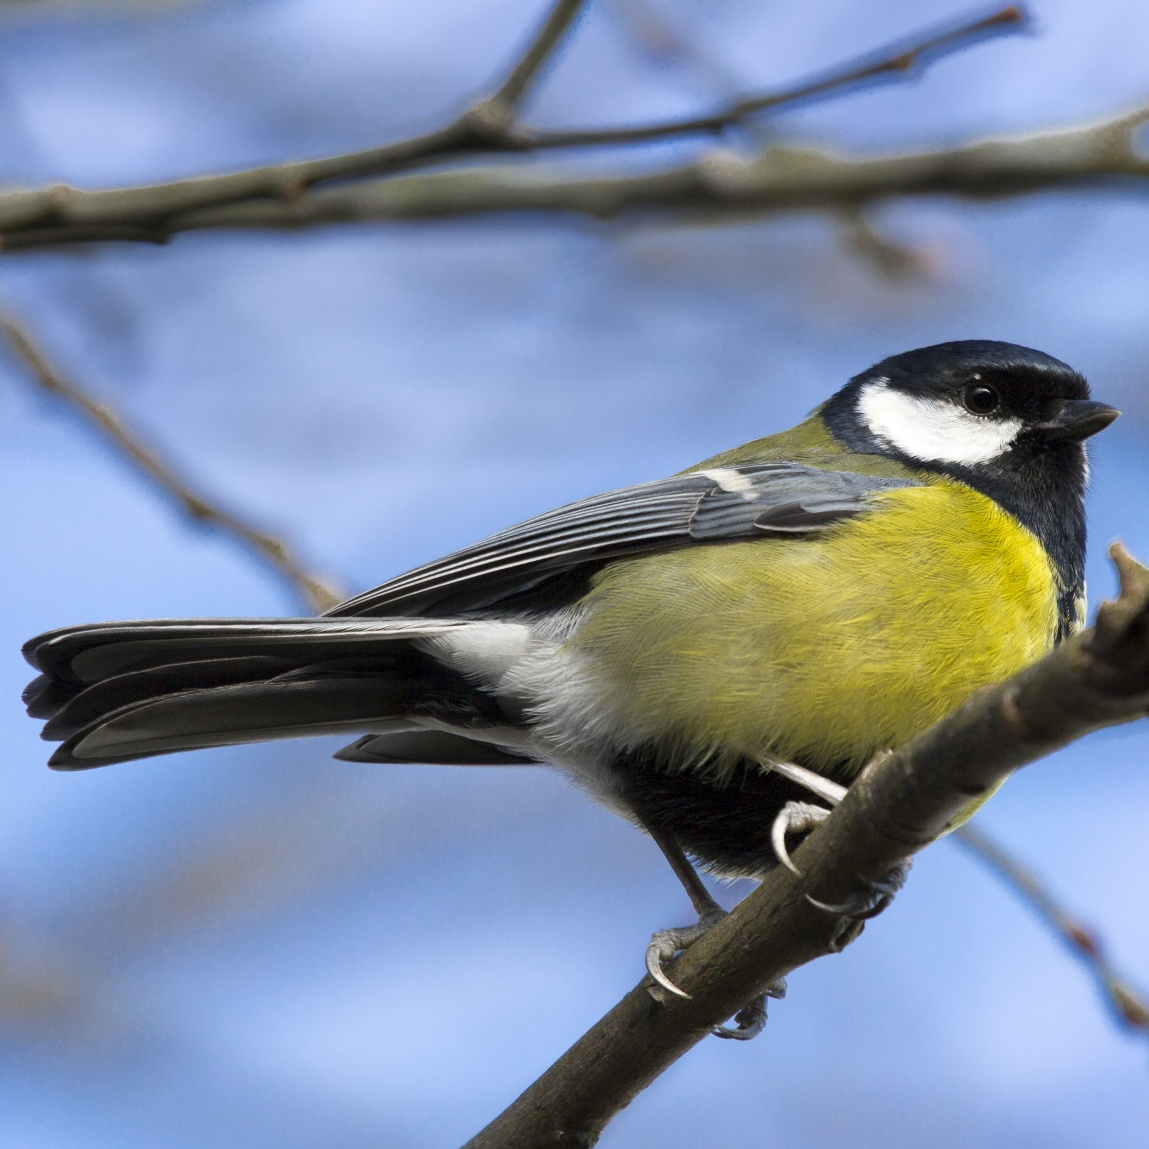
\includegraphics[width=\matpicw]{gt} & 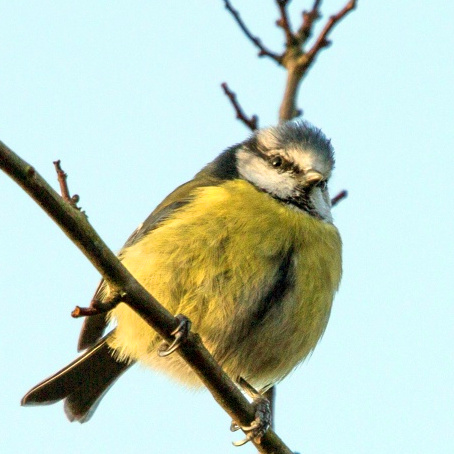
\includegraphics[width=\matpicw]{bt}&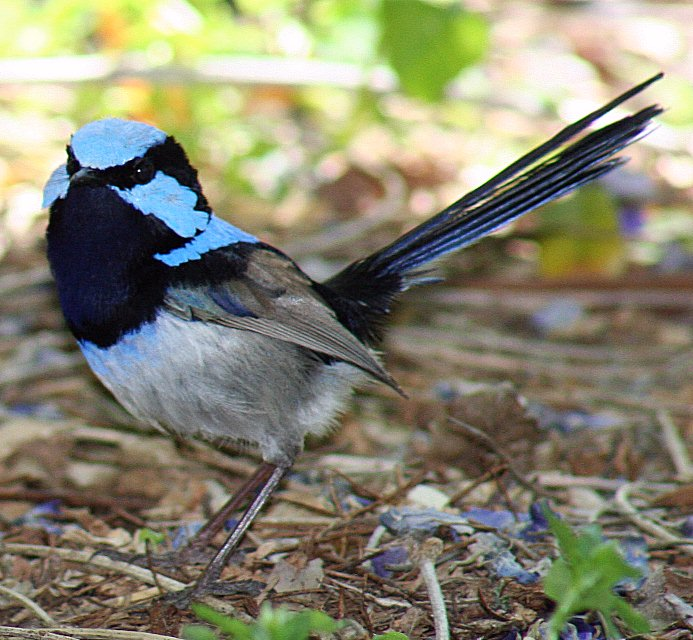
\includegraphics[width=\matpicw]{sfw} 
	   \end{tabular}
	  };
          
          \node[anchor=south west] (zih2) at (box.south west) {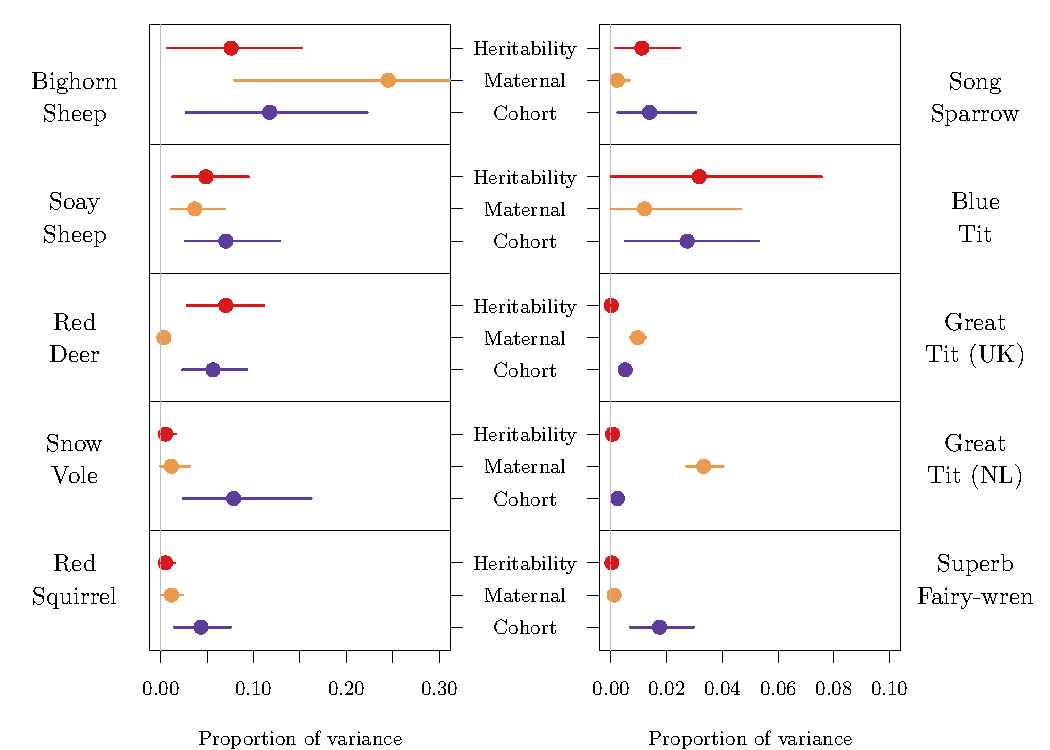
\includegraphics[width=24cm]{Rgraph/zih2.pdf}};
          %\node[anchor=north] (zih2com) at (zih2.south) {Heritabilities are small on the scale of the data\dots};
          \node[anchor=south west] (commh2) at ($(zih2.north west)+(1,-0.7)$) { \parbox{74cm}{
          Preliminary models suggest small heritabilities of fitness on the data-scale (average 2.4\%). Cohort effects, maternal effects and stochasticity dominate variation. However, credibility intervals of $V_A(\omega)$ exclude 0 in 5 out of 10 populations, and the posterior mode exceeds $0.1\%$ in all of them, suggesting widespread on-going evolution. 
          }
          };
          
          \node[anchor=west] (ziva) at (zih2.east) {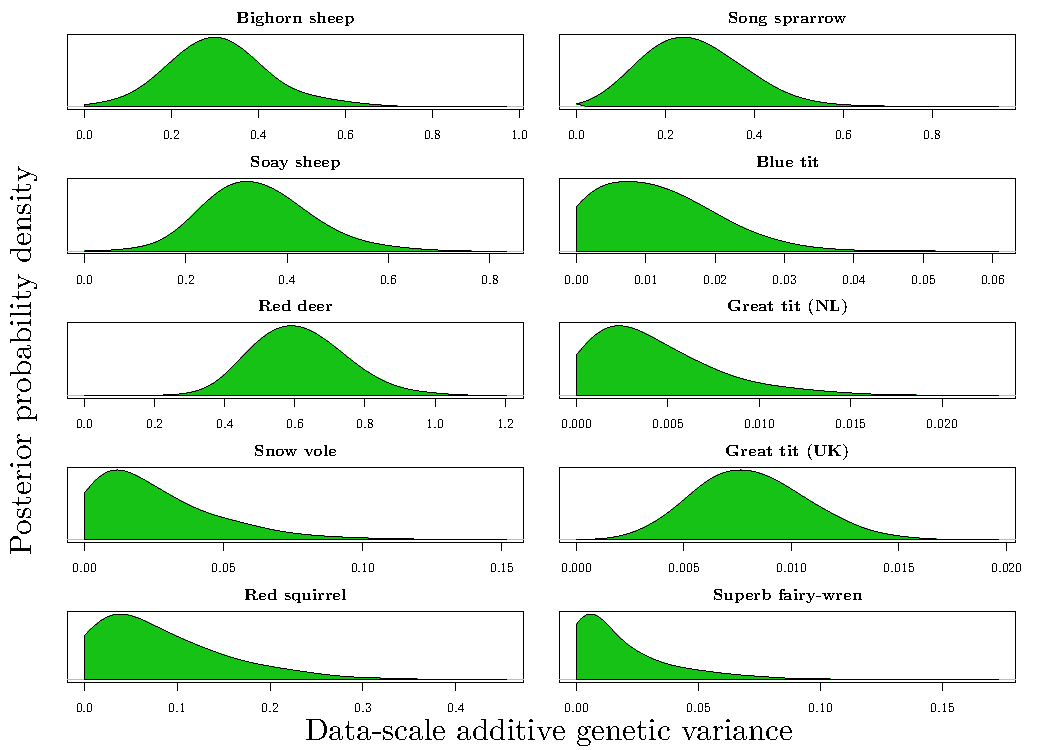
\includegraphics[width=24cm]{Rgraph/ziva.pdf}};
          \node[anchor=west] (com) at ($(ziva.east)+(-0.5,0)$) { \parbox{25.5cm}{\textsc{Next, we will explore:}
          \begin{itemize}
           \item Influence of priors on estimation
           \item Influence of missing data and imigration
           \item Sex-specific fitness. Does cross-sex genetic correlation constrain or enhance evolution?
           \item Relative importance of ZI, Poisson and their covariance
           \item Significance for population dynamics
          \end{itemize}

          }
          };
	  %\node[anchor=north] (zivacom) at (ziva.south) {\dots but that is irrelevant to the rate of evolution.};
                    
   \coordinate (currenty) at ($(box.south)-(yshift)$);
%%%%%%%%%%%%%%%%%%%%%%%%%%%%%%%%%%%%%%%%%%%%%%%%%%%%%

          
 %%%%%%%%%%%%%%%%%%%%%%%%%%%%%%%%%%%%%%%%%%%%%%%%%%%%%%%%%%%%%%%%%%%%%%%%%%%%%%%

    \node[anchor=north, rounded corners=15pt, fill=titledrawcolor] (qrw) at ($(currenty) + (-34,0)$) {
\includegraphics[width=8cm]{qrwebsite}};
    \node[anchor=north, rounded corners=15pt, fill=titledrawcolor] (qrgit) at ($(currenty) + (34,0)$) {
\includegraphics[width=8cm]{QRvawiswow}};
    \node[anchor=center] (web) at ($(qrw.north)+(0,0.7)$) {\textbf{\color{colorone!80!black}{Website}}};
    \node[anchor=north] (webadd) at ($(qrw.south)+(0,0.3)$) {\smallest{\color{colorone!80!black}{timotheenivalis.github.io}}};
    \node[anchor=center] (git) at ($(qrgit.north)+(0,0.7)$) {\textbf{\color{colorone!80!black}{R and \LaTeX code}}};
    \node[anchor=north] (gitadd) at ($(qrgit.south)+(0,0.3)$) {\smallest{\color{colorone!80!black}{github.com/timotheenivalis/VAWisWOW}}};

		
%%%%%%%%%%%%%%%%%%%%%%%%%%%%%%%%%%%%%%%%%%%%%		
   \Endblock{($(web.east)+(2,-4.7)$)}{57}{\hspace{25cm}\color{colorone}{\textsc{Co-authors:}}}{ 
   {\footnotesizeminus Josephine Pemberton, Tim Clutton-Brock, Marco Festa-Bianchet, David Coltman, Fanie Pelletier, Andrew McAdam, Stan Boutin, Anne Charmantier,
C\'eline Teplistky, Christophe de Franceschi, Erik Postma, Glauco Camenisch,
Marcel Visser, Ben Sheldon, Simon Evans, Lars Gustafsson,
Jane Reid, Matthew Wolack, Peter Arcese \& Andrew Cockburn} \\

{\color{colorone}{\**} Fisher's theorem relies on stringent assumptions, or alternatively on a specific meaning of evolution. In the absence of competition and gene-by-environment interactions, $V_A(\omega)$ is the increase in expected population growth rate. This clean link between evolution and demography probably doesn't apply (for long) in nature.}
  }
	
\end{tikzpicture}
  \end{document}
